\section{Simulation}

\hspace{\parindent} In parallel to the design, we simulated the operation of the robot using Matlab, Simulink and python. The work explained from now on is done on the last prototype presented in the previous section. However, the principle applied has been the same throughout the project. The simultaneous work was important in order to anticipate the delays due to the manufacturing of the robot. 

\subsection{Robot kinematics}

\textbf{Definition :} Given a vector $x=[x_1 x_2 x_3]^T \in \mathbb{R}^3$, we define : 
\begin{center}
    $[x] = \begin{bmatrix}
        0 & -x_3 & x_2 \\
        x_3 & 0 & -x_1 \\
        -x_2 & x_1 & 0 \\
    \end{bmatrix}$
\end{center}

\noindent\textbf{Definition :} Given two vectors $x$ and $y$ in $\mathbb{R}^3$, we define : $x\times y = [x]\cdot y$

\bigbreak

\noindent\textbf{Definition :} For a joint, we define the pitch $h = \frac{v}{w}$ with v : the linear speed and w the angular speed

\bigbreak

\noindent\textbf{Definition :} The screw is a $6\times1$ vector that represent the angular velocity when $\dot{\theta}=1$ and the linear velocity of the origin when $\dot{\theta}=1$. $S = \begin{bmatrix} s_w\\s_v\end{bmatrix}$ with $s_v = hw-s_w\times q$ where h is the pitch and q is a point on the 

\noindent\textbf{Definition :} For a given reference frame, a screw axis S is written as 
\begin{center}
    $S=\begin{bmatrix}
        s_w\\s_v
    \end{bmatrix}$
\end{center}
where either (i) $\|s_w\|$ = 1 or (ii) $\|s_w\|$ = 0 and $\|s_v\|$ = 1. If the pitch is finite ($h$ = 0 for a pure rotation), then $s_v = hs_w-s_w\times q$ where q is a point on the axis of the screw

\bigbreak

The figure below shows the kinematics schema of the robot. The figure defines an \{s\} frame at the bottom, an \{e\} frame at the end effector position and a \{c\} frame at the camera position. The robot is at is home configuration. The joint are represented with the rotation (positive rotation about the axes is by the right hand rule).

\bigbreak 

The parameters can be found with Onshape and are listed below: 

\begin{center}
    \fcolorbox{black}{white}{
        \begin{minipage}{0.8\linewidth}
            $L_0 = 0.069m$ \hspace{3cm} $d_0 = 0m$ \hfill $h_0 = 0.06m$ \\
            $L_1 = 0.116m$ \hspace{3cm} $d_1 = 0.018m$ \\ 
            $L_2 = 0.16m$ \hspace{3.2cm} $d_2 = 0.042m$ \\ 
            $L_3 = 0.155m$ \hspace{3cm} $d_3 = 0.01413m$ \\ 
            $L_c = 0.053m$ \hspace{3cm} $d_c = 0.0105m$ \hfill $h_c = 0.0815m$ \\
            $L_e = 0.2377m$ \hfill $d_e = 0.0105$ \hfill $h_e = 5.10^{-5}m$ \\
        \end{minipage}
    }
\end{center}

\begin{figure}[ht]
    \centering
    \includegraphics[width=0.8\textwidth]{images/kinematics\_schema.png}
    \caption{Kinematics schema}
    \label{fig:mesh10}
\end{figure}
\FloatBarrier

\bigbreak

We can then define $M_c$ and the $M_e$ the transformation matrix ($T_{sc}$ and $T_{se}$) when the robot is at its home configuration. 

\bigbreak
\begin{center}
    $
    M_c = \begin{bmatrix}
        0 & 0 & 1 & -h_0-L_3-h_c\\
        0 & -1 & 0 & d_1-d_2+d_3+d_c\\
        1 & 0 & 0 & l_0+l_1+l_2+l_c\\
        0 & 0 & 0 & 1
    \end{bmatrix}
    $
    and
    $
    M_e = \begin{bmatrix}
        0 & 0 & 1 & -h_0-L_3-h_c\\
        0 & -1 & 0 & d_1-d_2+d_3+d_c\\
        1 & 0 & 0 & l_0+l_1+l_2+l_c\\
        0 & 0 & 0 & 1
    \end{bmatrix}
    $
\end{center}

\subsubsection{Base frame}

\hspace{\parindent} In this subsection we study the kinematics parameters in the base frame \{s\}. It will be the one used in the followings sections.

\bigbreak

The rotation axis $S_{w_i}$ of each joint  in \{s\} are : 
\begin{center}
    $S_{w_1} = \begin{bmatrix} 0 \\ 0 \\ -1\end{bmatrix}$,
    $S_{w_2} = \begin{bmatrix} 0 \\ 1 \\ 0\end{bmatrix}$,
    $S_{w_3} = \begin{bmatrix} 0 \\ -1 \\ 0\end{bmatrix}$,
    $S_{w_4} = \begin{bmatrix} 0 \\ -1 \\ 0\end{bmatrix}$,
\end{center}

\bigbreak

We can also write the position of each joint  $q_1,q_2,q_3,q_4,q_c,q_e$ in \{s\}. Lining up the position as columns, we get : 

\begin{center}
    $
    \begin{bmatrix}
        -h_0 & -h_0 & -h_0 & -h_0-L_3 & -h_0-L_3-h_c & -h_0-L_3-L_e  \\
        0 & d_1 & d_1-d_2 & d_1-d_2+d_3 & d_1-d_2+d_3+d_c & d_1-d_2+d_3+d_e \\
        L_0 & L_0+L_1 & L_0+L_1+L_2 & L_0+L_1+L_2 & L_0+L_1+L_2+L_c & L_0+L_1+L_2+h_e \\
    \end{bmatrix}
    $
\end{center}

\bigbreak

There are all pure rotation joint, using the position, the rotation axis and the formula define in above we can calculate the screw axis $S_1,S_2,S_3,S_4$ in \{s\}.. Lining up them as columns, we get : 

\begin{center}
    $S_{list} = 
    \begin{bmatrix}
        0 & 0 & 0 & 0 \\
        0 & 1 & -1 & -1 \\
        -1 & 0 & 0 & 0 \\
        0 & -L_0-L_1 & L_0+L_1+L_2 & L_0+L_1+L_2 \\
        -h_0 & 0 & 0 & 0 \\
        0 & -h_0 & h_0 & h_0+L_3
    \end{bmatrix}
    $
\end{center}

\subsubsection{End effector frame}

\hspace{\parindent} In this subsection we study the kinematics parameters in the end effector frame \{e\}. However, it is not the one that will be use later. 

\bigbreak

The rotation axis $S_{w_i}$ of each joint  in \{e\} are : 
\begin{center}
    $S_{w_1} = \begin{bmatrix} -1 \\ 0 \\ 0\end{bmatrix}$,
    $S_{w_2} = \begin{bmatrix} 0 \\ -1 \\ 0\end{bmatrix}$,
    $S_{w_3} = \begin{bmatrix} 0 \\ 1 \\ 0\end{bmatrix}$,
    $S_{w_4} = \begin{bmatrix} 0 \\ 1 \\ 0\end{bmatrix}$,
\end{center}

\bigbreak

We can also write the position of each joint  $q_1,q_2,q_3,q_4,q_c,q_e$ in \{e\}. Lining up the position as columns, we get : 

\begin{center}
    $
    \begin{bmatrix}
        -h_e-L_2-L_1 & -h_e-L_2 & -h_e & -h_e & -h_e+L_c & 0  \\
        d_e+d_3-d_2+d_1 & d_e+d_3-d_2 & d_e+d_3 & d_e & d_e-d_c & 0 \\
        L_e+L_3 & L_e+L_3 & L_e+L_3 & L_e & L_e-h_c & 0 \\
    \end{bmatrix}
    $
\end{center}

\bigbreak

There are all pure rotation joint, using the position, the rotation axis and the formula define in above we can calculate the screw axis $B_1,B_2,B_3,B_4$ in \{e\}.. Lining up them as columns, we get : 

\begin{center}
    $B_{list} = 
    \begin{bmatrix}
        -1 & 0 & 0 & 0 \\
        0 & -1 & 1 & 1 \\
        -1 & 0 & 0 & 0 \\
        0 & L_e+L_3 & -L_e-L_3 & -L_e \\
        -L_e-L_3 & 0 & 0 & 0 \\
        d_e+d_3-d_2+d_1 & h_e+L_2 & -h_e & -h_e
    \end{bmatrix}
    $
\end{center}

\subsection{URDF Format}

\hspace{\parindent} The Universal Robot Description Format (URDF) is an XML (eXtensible Markup Language) file format used by the Robot Operating System (ROS) to describe the kinematics, inertial properties, and link geometry of robots. A URDF file describes the joints and links of a robot:

\begin{itemize}
    \item \textbf{Joints :} Joints connect two links: a parent link and a child link. A few of the possible joint types include prismatic, revolute (including joint limits), continuous (revolute without joint limits), and fixed (a virtual joint that does not permit any motion). Each joint has an origin frame that defines the position and orientation of the child link frame relative to the parent link frame when the joint variable is zero. The origin is on the joint's axis. Each joint has an axis 3-vector, a unit vector expressed in the child link's frame, in the direction of positive rotation for a revolute joint or positive translation for a prismatic joint.
    \item \textbf{Links :} While the joints fully describe the kinematics of a robot, the links define its mass properties. These start to be needed in Chapter 8, when we begin to study the dynamics of robots. The elements of a link include its mass; an origin frame that defines the position and orientation of a frame at the link's center of mass relative to the link's joint frame described above; and an inertia matrix, relative to the link's center of mass frame, specified by the six elements on or above the diagonal. (Since the inertia matrix is symmetric, it is onlynecessary to define the terms on and above the diagonal.)
\end{itemize}

\bigbreak

This format will also be useful to build the Simulink model of the robot. Thankfully, the library \textbf{onshape-tp-robot} in python can transform Onshape design into an URDF model. It is very important that you have respected the rules explained in the last section. It will download the stl file of each part and create all the joint and the links from the main assemnly. The inertia matrices and the mass are also imported for each block. 

\bigbreak

As explain on the librairy documentation, you should create onshape API key (see onshape developer portal). It is recommended to store them on your bashrc or zshrc because the secret key will no longer be shown.

\bigbreak
\begin{center}
    \begin{minipage}{10cm}
        \fcolorbox{black}{Azure}{\parbox{\linewidth}{
            export ONSHAPE\_API=https://cad.onshape.com\\
            export ONSHAPE\_ACCESS\_KEY=Your\_Access\_Key\\
            export ONSHAPE\_SECRET\_KEY=Your\_Secret\_Key
        }}
    \end{minipage}
\end{center}

\bigbreak

Then, you should create a folder where you want your urdf file to be construct and write a config.json file:
\begin{commandshell}
    mkdir -p robot\_urdf && touch robot\_urdf/config.json
\end{commandshell} 

\bigbreak
The config file must contain at least the following fields :
\begin{center}
    \begin{minipage}{8cm}
        \fcolorbox{black}{Azure}{\parbox{\linewidth}{
            \{\\
                \hspace*{0.8cm}"documentId": "document-id",\\
                \hspace*{0.8cm}"assemblyName": "onshape assembly",\\
                \hspace*{0.8cm}"outputFormat": "urdf"\\
            \}
        }}
    \end{minipage}
\end{center}

The documentId is the number (below XXXXXXXXX) you can find in Onshape URL:
\\https://cad.onshape.com/documents/XXXXXXXXX/w/YYYYYYYY/e/ZZZZZZZZ.

\bigbreak

Once this is done, if you properly installed and setup your API key, just run the following command. It will create an urdf file and put the stl file in the folder.
\begin{commandshell}
    onshape-to-robot robot_urdf
\end{commandshell} 

\bigbreak

The file will contains only the joints define in the final assembly. This is why you need subassemblies with the fixed part. As we can see on the extract below, the camera has a fixed joint with the hand. Also, it downloads all the stl files and describes the visual position of each. However, it has only one global parameter for each subassemblies that define the inertia.

\begin{figure}[ht]
    \centering
    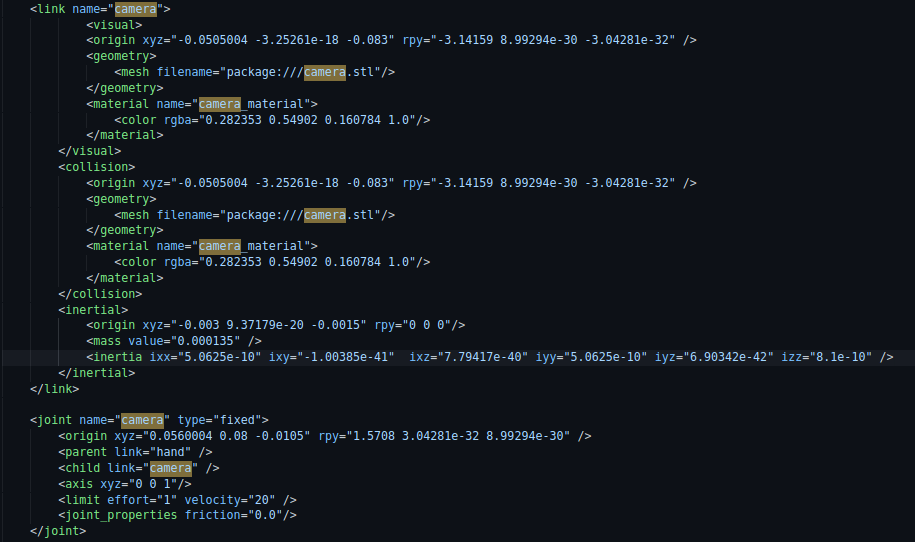
\includegraphics[width=0.8\textwidth]{images/urdf.png}
    \caption{URDF file extract}
    \label{fig:mesh11}
\end{figure}
\FloatBarrier

\subsection{Forward kinematics}
\subsubsection{Matlab simulation}

\subsubsection{Python simulation}

\subsection{Inverse kinematics}
\subsubsection{Matlab simulation}

\subsubsection{Python simulation}

\subsubsection{Torque Study}
\subsubsection{General principal}

\subsubsection{Joint results}

\subsubsection{Hardware choices}
